\section{Task}

\subsection{Understanding the light design problem} \label{understanding}

\textbf{Step 1. Setting the scenario}
\begin{itemize}
    \item In the \textit{Scene} tab, set the location to Ålesund. For this task, consider the path marked by the red line in the lower-left corner of Figure \ref{path}. 
    \begin{figure}[H]
    \centering
    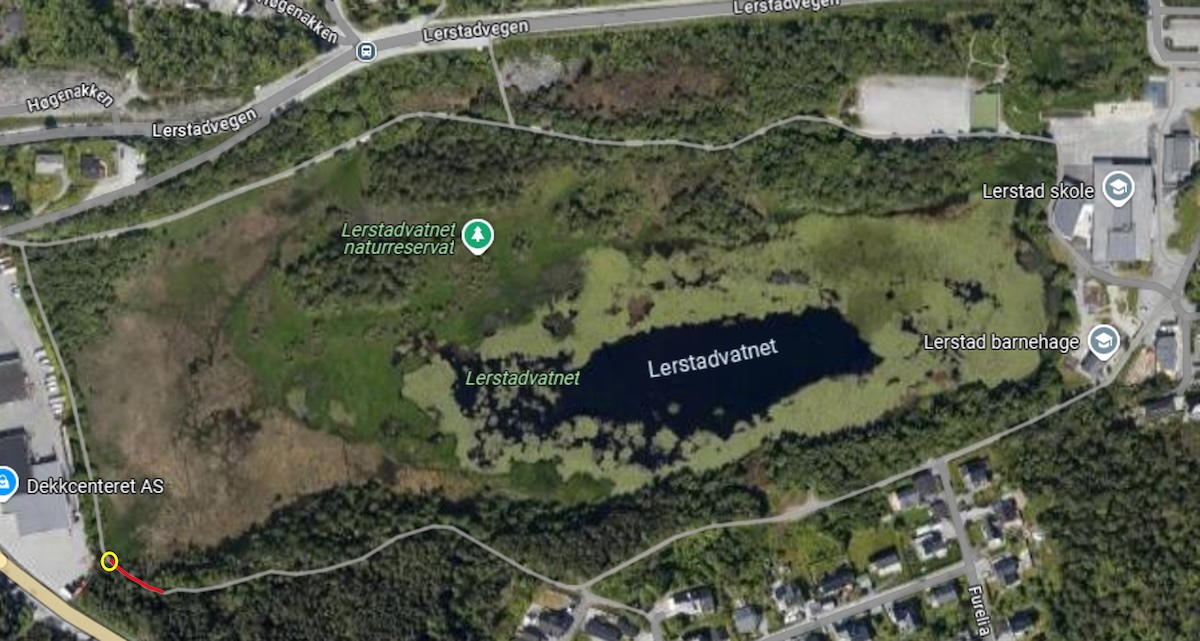
\includegraphics[width=0.75\textwidth]{Images/path.jpg}
    \caption[The analyzed path in Ålesund]{The analyzed path in Ålesund, the path marked by the red line in the lower-left corner}
    \label{path}
    \end{figure}
    \item Adjust the settings as follows: date to 25-December-2024, time to 16:30, clouds to \textit{sparse}, weather to 0.5 \textit{snow} and 0,5 \textit{fog}. Figure \ref{setup} shows a view from the path shown in the yellow circle of Figure \ref{path}. 
    \begin{figure}[H]
    \centering
    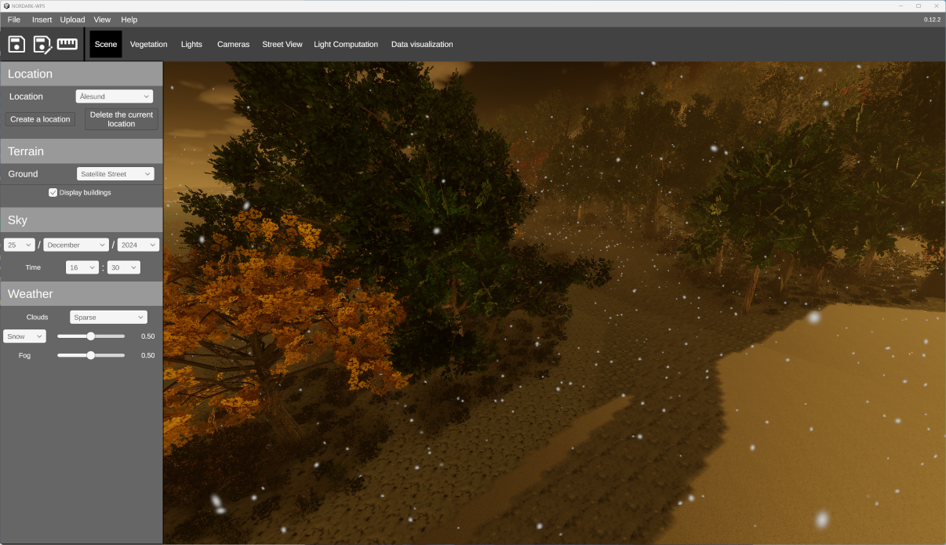
\includegraphics[width=0.75\textwidth]{Images/setup.jpg}
    \caption[The view of the analyzed path]{The view of the analyzed path}
    \label{setup}
    \end{figure}
\end{itemize}

\textbf{Step 2. Assessing the luminance condition}
\begin{itemize}
    \item By default, no light poles are designed on this path, as shown in the luminance graph in Figure \ref{line}.
    \begin{figure}[H]
    \centering
    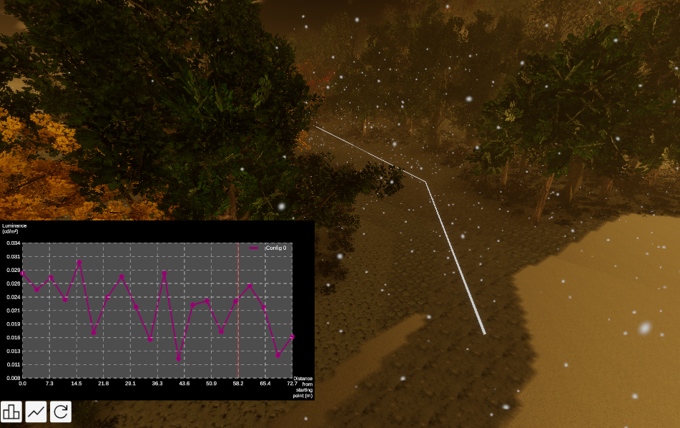
\includegraphics[width=0.75\textwidth]{Images/line.jpg}
    \caption[The luminance graph of the analyzed path, without light pole]{The luminance graph of the analyzed path, without light pole}
    \label{line}
    \end{figure}
    \item To generate this luminance graph, go to the \textit{Light Computation} tab, draw a line along the path by clicking on \textit{Create measure line manually}. Use left-click to start a new line and the right-click to finish the line. Then, check \textit{Display Graph} box to visualize the luminance graph along the drawn line. To save the results, export them by clicking \textit{Export (GeoJSON)} or \textit{Export (CSV)}, name the file (for example: result1). To save the current situation, go to file, and click save, name the file (for example: test1)
\end{itemize}

\subsection{Designing light interventions} \label{designing}

Using the same setup from the previous task in \ref{understanding} -- where no light poles were present on the path -- this task focuses on designing light poles along the path and comparing the results. By analyzing luminance across different setups, you can develop an optimized lighting model using Nordark digital twin. Various what-if scenarios can be explored in this digital twin before proceeding with installation. 

\textbf{Step 1. Creating light poles on the path}
\begin{itemize}
    \item In the \textit{Lights} tab, click \textit{Add}, then left click to place the pole. Adjust its height and rotation, choose the type and IES file.
    \item If you feel that there is not enough light poles on the path, add new ones by pressing "I" or clicking \textit{add} in the \textit{Lights} tab. An example is made with six light poles on the path, as seen in Figure \ref{six}.
    \begin{figure}[H]
    \centering
    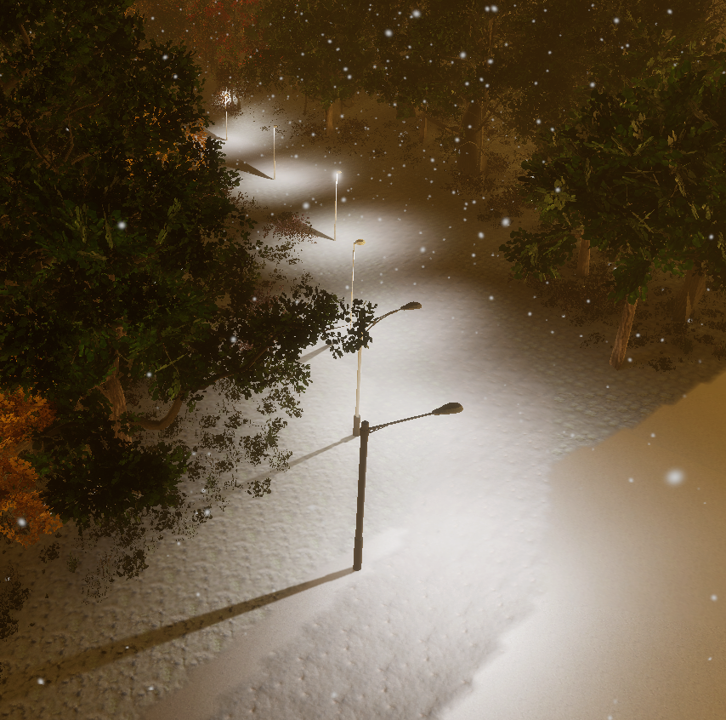
\includegraphics[width=0.75\textwidth]{Images/six.jpg}
    \caption[An example of six designed light poles]{An example of six designed light poles}
    \label{six}
    \end{figure}
\end{itemize}

\textbf{Step 2a. Comparing luminance graphs}
\begin{itemize}
    \item Go to \textit{Light Computation} tab, check the \textit{Display graph} box, then click the refresh button below the graph.
    \item To compare luminance graphs, click \textit{Import results} within the \textit{Line Visualization} column, then select the file "result1". Two luminance graphs can be seen in Figure \ref{compare}: the red line represents the new design with six light poles, while the green line represents the path without light pole (the imported one).
    \begin{figure}[H]
    \centering
    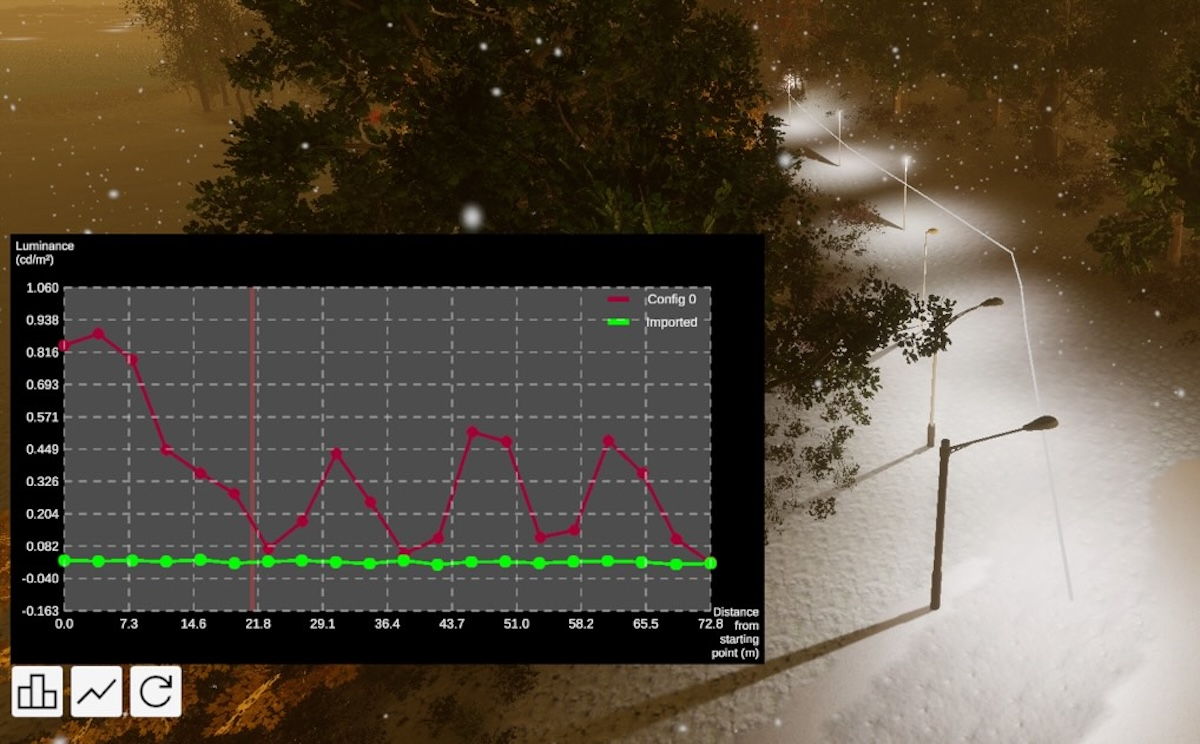
\includegraphics[width=0.75\textwidth]{Images/compare.jpg}
    \caption[Comparison on luminance graphs]{Comparison on luminance graphs: the red line represents the new design with six light poles, while the green line represents the path without light pole.}
    \label{compare}
    \end{figure}
\end{itemize}

\textbf{Step 2b. Comparing the luminance maps}
%\index{Luminance maps|comparing}
\begin{itemize}
    \item Go to \textit{Light Computation} tab, on the \textit{Configurations} column, set \textit{number of contributions} to 2.
    \item On the \textit{Scene config}, click the \textit{Browse} button, then select the saved file "test1", then check the \textit{Split screen} box.
    \item Check the \textit{Display luminance map} within the \textit{Luminance Map} column. The comparison result are shown in Figure \ref{compare_maps}.
    \begin{figure}[H]
    \centering
    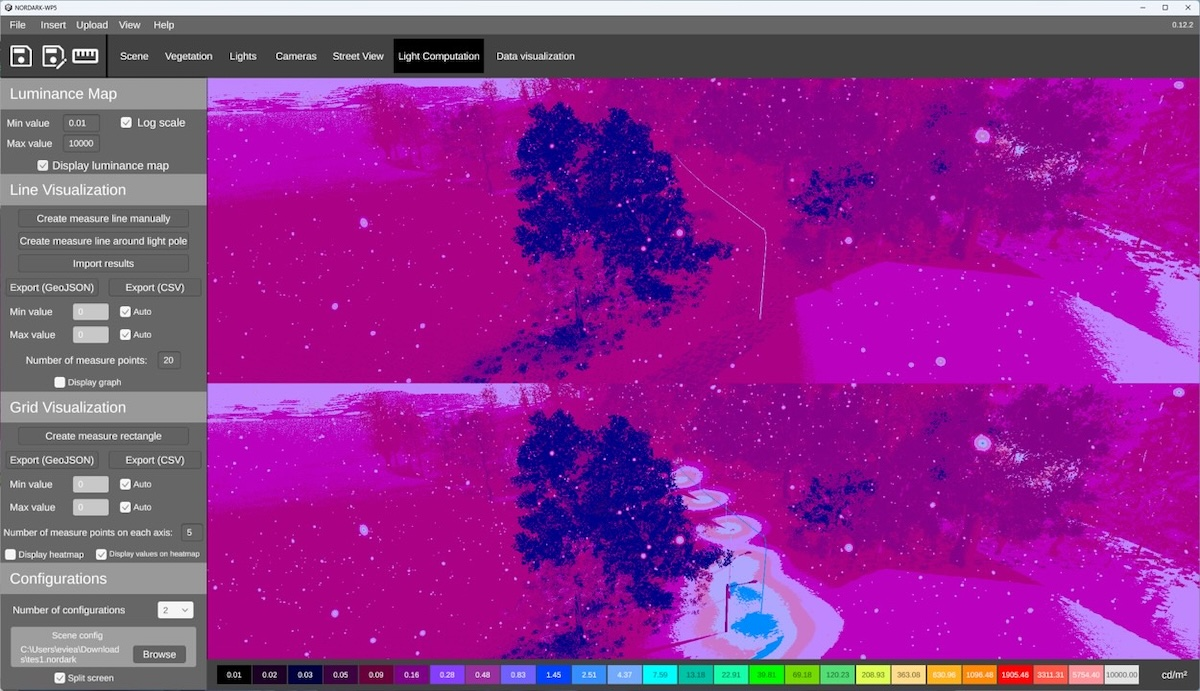
\includegraphics[width=0.75\textwidth]{Images/compare_maps.jpg}
    \caption[Comparison on luminance maps]{Comparison on luminance maps: Top section represents the path without light pole, while bottom section represents the new design with six light poles.}
    \label{compare_maps}
    \end{figure}
\end{itemize}



\subsection{Converting data from CSV format to Geojson for Light Computation} \label{converting}

The Nordark digital twin only supports geojson format to be imported, therefore, the original data needs to converted to the geojson file. Given that GeoJSON is a format for encoding a variety of geographic data structures, the original file requires information regarding location. It can be as a Point or a Linestring with latitude and longitude. There are two ways to find latitude and longitude information: (i) using Google Maps, and (ii) through the digital twin. For example, to find the coordinates of the red line shown in Figure \ref{setup}, open Google Maps and locate the exact spot. Then, right-click on the location; the first row that appears will display a pair of numbers in the format [latitude, longitude]. Repeat this process to mark multiple points along the red line in Figure \ref{setup}.

The other way to find latitude and longitude information is by using the digital twin through the \textit{Light Computation} feature. First, draw a line along the path you want to analyze (see Section \ref{Computation_tab} for how to draw a line). Then, check the \textit{Display Graph} box to show the luminance graph along that line. Click \textit{Export (CSV)} to save the data. When you open the CSV file, you will see columns for latitude, longitude, altitude, and distance from the starting point (in meters). This lets you get the coordinates for any location where you draw the line.

When you look at the saved CSV file, you can see the format needed for the digital twin to read the data. The file includes the following columns: latitude, longitude, altitude (m), distance from origin (m), luminance (cd/m²), ground (Path/Forest), and config. In the GeoJSON format, latitude, longitude, and altitude (m) are grouped under a feature called geometry. The other values are listed as properties that belong to that geometry.

Through the observation on the saved CSV file, you see the information format that is required for the digital twin to be able to read. The format is the column list, namely latitude, longitude, altitude (m), distance from origin (m), luminance (cd/m2), ground (Path/Forest), and config. On geojson format, the latitude, longitude, and altitude (m) are represented as a feature called "geometry". While the rest are properties that represent the information belonging to a geometry. 

To compare how the same data looks in both CSV and GeoJSON formats, use the \textit{Light Computation} feature. Draw a line, display the graph, then export the results in both CSV and GeoJSON formats. Open both files to compare them. You will see how the columns in the CSV file match the structure of the GeoJSON file, including the feature collection, features, and properties. By understanding the similarities and differences between the two formats, you will be able to format your own Excel or CSV file correctly. Once your CSV file includes all the required columns, you can use our Python script below to convert it into a GeoJSON file. This python script is also provided as a file named "convert\_CSV\_to\_Geojson.py".

\begin{lstlisting}[language=json,numbers=none,caption={Python script to convert CSV file to geojson format},captionpos=b]
import pandas as pd
import json
import os

*@\highlight{\# File paths}@*
csv_path = r'D:\Project\case3.csv' *@\highlight{\# Change this path based on where you saved the CSV file}@*
geojson_path = r'D:\Project\case3.geojson'  *@\highlight{\# Change this name for a different output file}@*

*@\highlight{\# Read the CSV file}@*
df = pd.read_csv(csv_path)

*@\highlight{\# Build GeoJSON structure}@*
geojson = {
    "type": "FeatureCollection",
    "features": []
}

for _, row in df.iterrows():
    feature = {
        "type": "Feature",
        "geometry": {
            "type": "Point",
            "coordinates": [
                row['longitude'],
                row['latitude'],
                row['altitude(m)']
            ]
        },
        "properties": {
            "luminance": row['luminance(cd/m2)'],
            "ground": row['ground'],
            "distanceFromOrigin": row['distanceFromOrigin(m)'],
            "config": row['config']
        }
    }
    geojson["features"].append(feature)

*@\highlight{\# Write to GeoJSON file}@*
with open(geojson_path, 'w') as f:
    json.dump(geojson, f, indent=2)
\end{lstlisting}

An example CSV file is provided for the case described in Section \ref{comparing}. This file, named "case3.csv", contains light measurements from light poles PR1 to PR8. To convert this CSV file, enter the file name and path into the csv\_path in the Python script.

The script uses the pandas library. If you haven't installed Python yet, please do so first. Then, open the Command Prompt and run the following command to install pandas: pip install pandas. Next, navigate to the folder where your script is located. For example: cd C:\\Desktop\\Project. Then run the script with: python convert\_csv\_to\_geojson.py. Here are some key points about how the script works:
\begin{itemize}
    \item Ensure the CSV file is saved and closed before running the script.
    \item The script expects the column names to match exactly (including parentheses and case).
    \item The coordinates are formatted as [longitude, latitude, altitude], which is standard for GeoJSON.
    \item The output GeoJSON will have each row as a Point feature with all the specified properties.
    \item To use a different name, simply modify the geojson\_path variable.
\end{itemize}

\subsection{Formatting data to Geojson for the data visualization} \label{formatting}

As mentioned earlier, the GeoJSON format requires geometry information regarding the latitude and longitude. You can get these coordinates by following the steps in Section \ref{converting}. Each geometry can represent a different category you want to visualize. For example: in Section \ref{env}, each geometry represents one of three lighting conditions. In Section \ref{questionnaire}, geometries are used in two ways: (i) to represent different questions, and (ii) to represent different answers. How you define each geometry depends on the purpose of your visualization.

As explained in Section \ref{datavis}, the data visualization feature works by scaling values between 0 (worst) and 1 (best). So, before visualizing your data, you need to scale your values to fit within this range. Then, list your variables and include them as properties in the GeoJSON file.

An example of this process is shown in Section \ref{env}, using a task from WP1. Take a look at the original file WP1-Ålesund data\_Day-Head torches.xlsx and the converted file EnvironmentalPsychology.geojson. In the original file, the \textbf{mean} values are rated from 1 to 5. These must first be scaled to fall between 0 and 1. In the converted GeoJSON file, you’ll see three geometries —each one represents a column from the Excel file: daylight, head torch regular, and head torch customized. Each row from the Excel file becomes a set of properties under each geometry in the GeoJSON file. By reviewing both files and understanding how the conversion is done, you can apply the same approach to your own data. 

You can also use the Python script mentioned earlier, with a few additional steps beforehand. First, you need to reformat your original file into a CSV format —this may involve switching the column headers to rows, or vice versa, depending on your data structure. Next, update the Python script by replacing the list of properties with your own variables. Also, make sure to double-check that the file paths in the script are correct.





